\documentclass[12pt, a4paper]{article}
\usepackage[print,sort]{standalone}
\usepackage[T1]{fontenc}
\usepackage[utf8]{inputenc}
\usepackage[english]{babel}
\usepackage{graphicx,float}
\usepackage{amssymb}
\usepackage{amsmath,cancel}
\usepackage{mathrsfs}
\usepackage{epstopdf}
\usepackage{subcaption}
\usepackage{slashed}
\usepackage{hhline}
\usepackage[margin=1.2in]{geometry}
\usepackage[hidelinks]{hyperref}
\usepackage{wrapfig}


\hfuzz=5pt


\begin{document}

\begin{titlepage}
\begin{center}
\vspace*{3cm}
\Huge
\textbf{Project 3} \\
\Large  
FYS4150 Computational Physics 
\vspace*{3cm} \\ 

Even S. Håland 
\vspace*{5cm} \\

\normalsize
\section*{Abstract}

The motion of the planets in the solar system is governed by gravitational forces between the planets 
and the sun, and between the planets themselves. This can be expressed mathematically as a set of coupled 
differential equation. In this project we solve these equations, mainly by using the velocity Verlet 
algorithm. When doing so we use an object oriented approach, and two classes are developed; a 
\textit{planet} class and a \textit{solver} class. We find that the problem can be solved in a quite nice 
and compact way, and we get quite good estimates of the planetary orbits.  

\end{center}
\end{titlepage}

\section{Introduction}

The concept of object oriented programming was invented in the mid 1960s at the Norwegian Computing 
Centre in Oslo\cite{OOP}, and can be a very powerful way of programming. This applies especially if 
you have e.g. an algorithm that you want to apply to a variety of similar systems. Instead of writing 
new code tailored to each system, you write the algorithm in a more general way that allows you to 
apply it to different systems. The systems we will study in this project consists of planets 
orbiting the Sun. We will simulate both a binary system (e.g. the Earth and the Sun), a three-body system 
(Earth, Sun and Jupiter), and eventually the full solar system. The magic of object orientation is that 
once you have written the algorithm it is very easy to jump between each of these systems. 

Two key concepts of object oriented programming is \textit{classes} and \textit{objects}. A class can be 
thought of as a set of variables and functions, while an object is an instance of the class. We 
say that the object inherits the functions and variables defined in the class. Two classes are written in 
this project, namely a planet class and a solver class, which will be discussed in more detail later. 

The first part of the report is a short theoretical introduction to how we model planetary motion using 
Newtons law of gravitation, followed by the procedure for discretizing the equations and a discussion of 
the algorithms. Then the main aspects and ideas of the programs are discussed, before the results are 
presented towards the end.  

\section{Modelling planetary motion}

Newtons law of gravitation states that the gravitational force between two objects, with mass $M$ and $m$
respectively, is given by 
\begin{align}
F_G = \frac{GMm}{r^2}, 
\end{align}
where $G$ is the gravitational constant and $r$ is the distance between the two objects. This is 
the "corner stone" of all calculations done in this project. 

\subsection{Earth-Sun system}

We start by considering a system with only two objects, namely the Sun (with mass $M_{\odot}$) and the 
Earth (with mass $M_{\text{ Earth}}$), and we assume that the Sun is fixed, so that the only motion we 
have to care about is that of the Earth. We also assume that the motion of the Earth is co-planar, 
and take this 
to be the $xy$-plane, with the Sun in the origin. When writing the programs and implementing the 
algorithm we actually work in $3D$, but extending from two to three dimensions is quite trivial.  

The forces acting on the Earth in the $x$- and $y$-direction are given by 
\begin{align*}
F_{G,x} = - F_G \cos\theta  = - \frac{GM_{\odot} M_{\text{Earth}}}{r^2}\cos\theta 
							= - \frac{GM_{\odot} M_{\text{Earth}}}{r^3}x 
\end{align*} 
and 
\begin{align*}
F_{G,y} = - F_G \sin\theta  = - \frac{GM_{\odot} M_{\text{Earth}}}{r^2}\sin\theta 
							= - \frac{GM_{\odot} M_{\text{Earth}}}{r^3}y,  
\end{align*}
where we have used the relations $x = r\cos\theta$ and $y = r\sin\theta$. From Newtons second law we know 
that the accelerations, $a_x$ and $a_y$, are given as 
\begin{align*}
a_x = \frac{d^2x}{dt^2} = \frac{F_{G,x}}{M_{\text{Earth}}} \quad \text{and} \quad 
a_y = \frac{d^2y}{dt^2} = \frac{F_{G,y}}{M_{\text{Earth}}}. 
\end{align*} 
We also know that the acceleration is the time derivative of the velocity, $v$, which again is 
the time derivative of the position, meaning that we can express the equations of motion as two 
coupled first order differential equations in each dimension:  
\begin{align}
v_x = \frac{dx}{dt}, \quad v_y = \frac{dy}{dt}, \quad 
a_x = \frac{dv_x}{dt} = -\frac{GM_{\odot}x}{r^3}, \quad a_y = \frac{dv_y}{dt} = -\frac{GM_{\odot}y}{r^3}.   
\label{eq:diff_eqs}
\end{align}
When extending to three dimensions we simply add two more equations like those above, simply 
replacing $x$ or $y$ by $z$. 

\subsection{Scaling of equations}

The next thing we want to do is to scale the equations appropriately. When working on an astronomical 
scale we prefer to work with years (yr) as the time unit and AU\footnote{Astronomical units; $1$ AU is
defined as the mean distance between the Earth and the Sun.} as the length unit. This means that we 
need to find some way of scaling the gravitational constant, $G$, to these units. 

If we assume the orbit 
of the Earth to be circular (which is very close to the truth), the acceleration is given as 
\begin{align*}
a = \frac{v^2}{r} = \frac{F_G}{M_{\text{Earth}}} = \frac{GM_{\odot}}{r^2} \quad \Rightarrow \quad 
v^2 r = GM_{\odot}, 
\end{align*}  
where $r = 1$ AU, while the velocity is 
\begin{align*}
v = 2\pi \:\: \text{AU/yr},   
\end{align*}
which means that 
\begin{align*}
GM_{\odot} = 4\pi^2 \:\: \text{AU}^3/\text{yr}^2,  
\end{align*}
which can be inserted in the equations of motion. In addition to this it is also 
convenient to scale the mass of the earth (and other planets) to the solar mass, i.e. we put 
$M_{\odot} = 1$, and scale other masses accordingly. We do this to decrease the chance of loosing 
numerical precision through round-off errors, as the planetary masses are quite large (see Table  
\ref{tab:planets}). 

\subsection{The solar system}

Once we know the form of the gravitational interaction it is quite easy to extend our system to include 
other planets, and eventually the full solar system. The general forces in the $xy$-planet  
between two planets with mass $M_a$ and $M_b$ are given by 
\begin{align*}
F_{G,x} = \frac{GM_aM_b}{r^3}\Delta x \quad \text{and} \quad F_{G,y} = \frac{GM_aM_b}{r^3}\Delta y, 
\end{align*}  
where $\Delta x$ and $\Delta y$ are the distances between the planets in $x$- and $y$-direction, and 
$r$ the absolute distance between them. When we want to model a system with several planets we simply 
add up the forces acting on each planet, and calculate the acceleration of a specific planet as 
the total force acting on it divided by its mass. The planets of the solar system are listed in Table 
\ref{tab:planets}, along with their masses and distances to the Sun.   

\begin{table}
\caption{Mass and distance to the Sun for the planets in the solar system. (Numbers taken from the 
project description.)}
\label{tab:planets}
\begin{center}
\begin{tabular}{ccc} \hline\hline
Planet & Mass (kg) & Distance to Sun (AU) \\ \hline 
Earth & $6\times10^{24}$ & $1$  \\
Jupiter & $1.9\times10^{27}$ & $5.20$  \\
Mars & $6.6\times10^{23}$ & $1.52$ \\
Venus & $4.9\times10^{24}$ & $0.72$ \\
Saturn & $5.5\times10^{26}$ & $9.54$ \\ 
Mercury & $3.3\times10^{23}$ & $0.39$ \\ 
Uranus & $8.8\times10^{25}$ & $19.19$ \\ 
Neptune & $1.03\times10^{26}$ & $30.06$  \\ 
Pluto & $1.31\times10^{22}$ & $39.53$ \\ \hline \hline
\end{tabular}
\end{center}
\end{table}

Before we start looking at how we should study this numerically there is one more thing that needs to 
be mentioned in this theoretical introduction. Newtonian mechanics is able to describe 
the planetary orbits quite well. It was however observed in the $1800$s that Mercury's 
perihelion precession was off by
$43''$ ($\sim 0.012^{\circ}$) per century (which is a very small deviation!) compared to the 
predictions from the Newtonian theory. However, in Einstein's general theory of relativity 
the gravitational force gets a small correction, and can be written as 
\begin{align*}
F_G = \frac{GM_{\odot}M_{\text{Mercury}}}{r^2}\left[ 1+ \frac{3l^2}{r^2c^2} \right], 
\end{align*} 
where $l=|\mathbf{r}\times \mathbf{v}|$ is the magnitude of the orbital angular momentum per unit mass and 
$c$ is the speed of light. Towards the end of the project we will see (spoiler alert!) that this 
correction actually is able to explain the observed perihelion precession!  

\section{Discretization and algorithms}

We would like to write a code that calculate updated positions for a system of planets as time 
passes. In order to do so we must, as usual, start by making a discrete approach to the problem. 
The discretization will only be shown for one dimension ($x$), since the procedure is completely
equivalent for the other dimensions. Time and position are discretized as 
\begin{align*}
&t  \rightarrow t_i = t_0 + ih \\
&x(t)  \rightarrow x(t_i) = x_i, 
\end{align*}   
with the time step, $h$, given by 
\begin{align*}
h = \frac{t_f - t_0}{n}.  
\end{align*}
Here $t_0$ and $t_f$ is the initial and final time respectively, $n$ is total number of time steps and 
$i$ runs from $1$ to $n$. 

Position and velocity after some time $t_i+h$ is given by Taylor expansion as 
\begin{align}
x_{i+1} & = x_i + hx_i' + \frac{h^2}{2}x_i'' + O(h^3) \nonumber \\ 
	    & = x_i + hv_i + \frac{h^2}{2}a_i + O(h^3)
\label{eq:Taylor_pos}	    
\end{align}
and 
\begin{align}
v_{i+1} & = v_i + hv_i' + \frac{h^2}{2}v_i'' + O(h^3) \nonumber \\
		& = v_i + ha_i + \frac{h^2}{2}v_i'' + O(h^3),  
\label{eq:Taylor_vel}
\end{align}
where $a_i$ is the acceleration, which for the Earth-Sun system is given in discrete form as  
\begin{align*}
a_i = \frac{F(x_i,t_i)}{M_{\text{Earth}}} = - \frac{GM_{\odot}x_i}{r_i^3}. 
\end{align*}
Based on these equations we will consider two methods for approximating positions and velocities.

The first one is the forward Euler (FE) method, which we get directly from the above equations, by only 
including terms from eqs. (\ref{eq:Taylor_pos}) and (\ref{eq:Taylor_vel}) up to $O(h^2)$: 
\begin{align*}
x_{i+1} & \approx x_i + hv_i \\ 
v_{i+1} & \approx v_i + ha_i 
\end{align*}


The second one is the velocity Verlet (VV) method, where we keep terms up to $O(h^3)$. This means that 
we are stuck with a second derivative of the velocity, which we want to get rid of. This is done by 
Eulers formula, so 
\begin{align*}
v_i'' \approx \frac{v_{i+1}'+v_i'}{h} = \frac{a_{i+1}+a_i}{h},  
\end{align*}
which leaves us with the following approximations for position and velocity: 
\begin{align*}
x_{i+1} & \approx x_i + hv_i + \frac{h^2}{2}a_i  \\
v_{i+1} & \approx v_i + \frac{h}{2}\left[ a_{i+1} + a_i  \right] 
\end{align*}

Notice that the VV algorithm require some more floating point operations (FLOPS) than FE. If we 
pre-calculate $\frac{h}{2}$ and $\frac{h^2}{2}$ we need $7$ FLOPS per time step for VV against $4$ with 
the FE method. However, 
we also need to calculate the forces acting on the planet in order to calculate the acceleration. This 
must be done twice for each time step in the VV loop and only once per time step in the FE loop. 

Both of these methods will be implemented in our code. However, the VV algorithm will be 
proven to work somewhat better than FE, so throughout most of the project we 
will stick to using the VV method.  

Notice that in order to get the algorithms started we need some initial values for position and 
velocity, i.e. $x_0$ and $v_0$, hence these kinds of problems are referred to as \textit{initial 
value problems}.   


\section{Code}

All code written for this project can be found in the following git repository: \vspace{0.5cm} \\ 
\fbox{
\href{https://github.com/evensha/FYS4150/tree/master/Project3/Programs}
{https://github.com/evensha/FYS4150/tree/master/Project3/Programs} } \vspace{0.5cm} \\ 
The most important files in this repository are:  
\begin{itemize}
\item \texttt{planet.cpp/planet.h}
\item \texttt{solver.cpp/solver.h}
\item \texttt{main.cpp}
\item Various (python) plotting scripts. 
\end{itemize}
Before going into the details of the code we should have a quick look at the main structure and purpose 
of the different programs and classes. 

Firstly we have two classes called \textbf{planet} (implemented in \texttt{planet.cpp} and 
\texttt{planet.h}) and \textbf{solver} (implemented in \texttt{solver.cpp} and \texttt{solver.h}). 
The main idea is that we let each planet we want to consider be an object of the planet class, 
which has properties like position, velocity, mass, and functions that can calculate other quantities 
for the planet. We then make an object of the solver class, and put our planets in to this object. 
The solver class contain functions that will solve our problem, i.e. by using forward Euler or 
velocity Verlet, in addition to other functions that could be useful. The main program (\texttt{main.cpp}) 
is used to initialize the necessary objects, and run the solver functions, while several different python 
scripts are used for plotting the results. The output from the programs is stored in 
the "Output" repository. However, one might not find all produced output files in the mentioned git 
repository, as some of the produced output files are quite large.  

In addition to the above described programs it is also worth mentioning that the git repository contains 
a \texttt{makefile}, used for compiling it all, and a file called \texttt{Planet\_data.txt}. The latter 
file contains necessary information about all the planets, i.e. mass and the positions and velocities 
we will use as initial values. The positions and velocities are taken from ref. \cite{NASA}.  

\subsection{The planet class}

The planet class has four public variables: 
\begin{itemize}
\item \texttt{mass:} The mass of the planet. 
\item \texttt{position:} Three dimensional double containing the coordinates of the planets position.
\item \texttt{velocity:} Three dimensional double containing the velocities of the planet in each 
dimension.
\item \texttt{name:} The name of the planet, given as a string.  
\end{itemize}
An object of this class can be initialized with a default initialization that sets all the variables to 
zero, and the name to "Planet". Alternatively it can be initialized with mass, positions, velocities and 
name. Positions and velocities can be given in either two or three dimension. 

Further the class contains the following functions (which all return a double): 
\begin{itemize}
\item \texttt{Distance(planet otherPlanet):} Take an other object of the planet class as input argument, 
and calculates the distance to this planet. 
\item \texttt{PotentialEnergy(planet otherPlanet):} Take an other object of the planet class as input, and 
calculates the planets potential energy with respect to the other planet.   
\item \texttt{xMomentum():} Calculates the planets momentum in the $x$-direction. 
\item \texttt{yMomentum():} Calculates the planets momentum in the $y$-direction. 
\item \texttt{AngularMomentum():} Calculates the magnitude of the orbital angular momentum per unit 
mass of the planet. 
\end{itemize}

\subsection{The solver class}

The solver class has the following public variables: 
\begin{itemize}
\item \texttt{mass:} Mass of the system you are studying. 
\item \texttt{G:} Gravitational constant, $4\pi^2$ by default. 
\item \texttt{beta:} Power of $r$ in the denominator of the gravitational force, i.e. 
$F_G \propto 1/r^{\beta}$. By default $\beta = 2$, but we will also study some variations of the 
gravitational force. 
\item \texttt{RelCorr:} Integer that indicates whether or not you want to add the previously discussed 
relativistic correction to the gravitational force:
\begin{itemize}
\item \texttt{0:} without relativistic correction (default). 
\item \texttt{1:} with relativistic correction. 
\end{itemize}  
\item \texttt{total\_planets:} Integer denoting the total number of planets in your system. 
\item \texttt{all\_planets:} Vector that contains the "planet objects" you have added to the solver class. 
\end{itemize}
The solver class is initialized either with a default initialization, or by specifying \texttt{RelCorr} 
or \texttt{beta} discussed above. The class contains the following functions: 
\begin{itemize}
\item \texttt{addPlanet(planet newplanet):} Takes an object of the planet class as input, and adds this 
object to the solver object, updating the total mass and number of planets in the system. 
\item \texttt{ForwardEuler(int integration\_points, double time,\\ int withOutput):} 
Takes number of integration points and the final time of your simulation (in years) as input, as well as 
an argument specifying whether or not you want to produce any output\footnote{By output it is here meant 
a file containing the positions we are calculating.}. (\texttt{1} if you want output, \texttt{0} if not.)
The function then runs through the time steps and the planets in you system, updating positions and 
velocities of the planets according to the forward Euler algorithm.
 
\item \texttt{VelocityVerlet(int integration\_points, double final\_time, \\ int withOutput):} Similar 
in structure to the forward Euler function, only this one is using the velocity Verlet method. A slight 
difference is however that the position of the perihelion of the orbit also can be calculated inside 
this function, which is useful when we are going to study Mercury's orbit. 
\item \texttt{GravitationalForce(planet \&Planet, planet \&other, double \&F\_x, \\ double \&F\_y, 
double \&F\_z, double beta, int RelCorr):} Calculates the gravitational forces between two specified 
planets in three dimensions.  
\item \texttt{PrintPositions():} Prints the current positions to the output file.    
\item \texttt{PrintNames():} Prints the names of all your planet objects to the output file. 
\end{itemize} 

\subsection{The main program and plotting}

The purpose of the main program is to initialize the needed planet objects and the solver, put the planets 
into the solver, and then run the relevant functions. The program takes number of time steps, 
final time of the simulation and name of the problem as input. 

Different solver objects are initialized, depending on which problem we want to consider. If we want to 
consider the full solar system the planets are initialized with data from the \texttt{Planet\_data.txt} 
file, which are stored in maps relating the variables to the corresponding planet.  

As mentioned, several different python scripts are used for plotting, depending on the situation and 
system we study. These scripts read the output files produced by the solver. (I realized towards 
the end of the project that it might also could be handy to write a class for the plotting, 
but unfortunately there was no time to do this.) 

\section{Results}

In this section all the results are presented. We start by doing some tests of the two algorithms, before 
we move on to simulating a three-body system and the full solar system. Finally we will (as promised) 
look at the perihelion precession of Mercury's orbit. 

\subsection{Testing the algorithms (Earth-Sun system)}

In order to test the programs and algorithms we have developed we start by considering the binary system 
with the Sun (fixed in the origin) 
and the Earth moving in a circular orbit, and we only consider two dimensions. In order for the Earth to 
get a circular orbit the magnitude of the velocity must be $v=2\pi$ AU/year (given $r = 1$ AU), so we 
initialize the system by putting $v_x = 0$ and $v_y = 2\pi$ AU/year. 

Figure \ref{fig:FE_vs_VV} shows comparisons of the orbits we get by using FE and VV 
over a period of $10$ years. In the upper plot we have chosen $10,000$ time steps, while in 
the lower plot we have $100,000$ time steps. We see from these plots that the orbits obtained by the 
VV looks very nice and stable in both cases, while the FE orbits are spiralling outwards. The spirals 
gets closer when we increase the number of time steps, but we see that the effect is still there. 

\begin{figure}
\centering
  	\begin{subfigure}[b]{1\textwidth}
	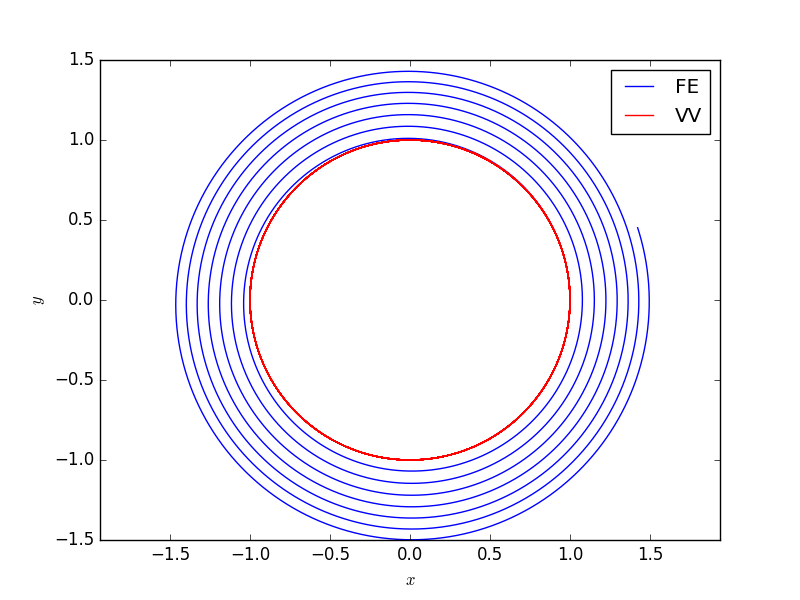
\includegraphics[scale=0.65]{../Programs/Output/FE_vs_VV_n=10000.png}
	\caption{$10,000$ time steps.}
	\end{subfigure} 	
  	\begin{subfigure}[b]{1\textwidth}
	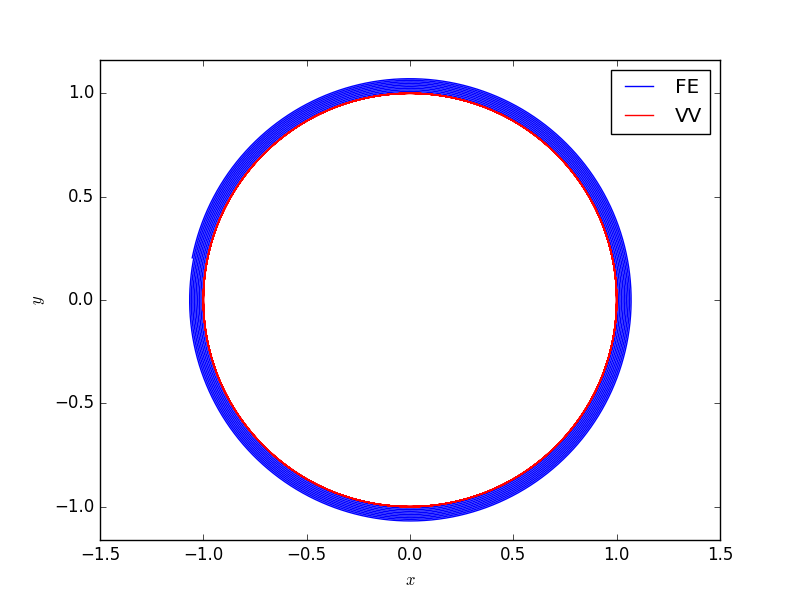
\includegraphics[scale=0.65]{../Programs/Output/FE_vs_VV_n=100000.png}
	\caption{$100,000$ time steps.}	
	\end{subfigure} 	
\caption{Orbits obtained by using forward Euler and velocity Verlet, when running over $10$ years.}
\label{fig:FE_vs_VV}
\end{figure} 

Another way of testing the algorithms is to consider conservation of some kinematic quantities. Since 
the orbits (in this test case) should be perfect circles the kinetic and potential energy should be 
separately conserved, since the velocity and distance to the sun should stay the same.
These two quantities are given as 
\begin{align*}
E_k = \frac{1}{2}M_{\text{Earth}}v^2 
\end{align*}
and 
\begin{align*}
E_p = - \frac{GM_{\odot}M_{\text{Earth}}}{r}
\end{align*}
respectively. Also, since the sun is fixed there should be no transfer of angular momentum, meaning that
also this quantity should be conserved. We will consider the magnitude of the angular momentum per unit 
mass, which is given as 
\begin{align*}
l = | \mathbf{r} \times \mathbf{v} |. 
\end{align*}
In Table \ref{tab:kinematics} these quantities are given for the initial state of the Earth, 
and after a $10$ years simulation with $10,000$ time steps for the two algorithms.
Notice that the calculations are done in the units we used for scaling the equations (i.e. AU, years and 
mass per $M_{\odot}$.) We see here that 
with the VV algorithm all of these are perfectly conserved, while non of them are conserved 
using the FE algorithm.  

\begin{table}[ht!]
\caption{Kinetic and potential energy, and angular momentum (per unit mass), calculated before we 
run the algorithms and after $10$ years and $10,000$ time steps of forward Euler and velocity Verlet. 
The quantities are calculated using the units discussed earlier.}
\label{tab:kinematics}
\begin{center}
\begin{tabular}{lccc}  
		& Kinetic energy & Potential energy & Angular momentum  \\ \hline 
Initial value   & $5.92\cdot10^{-5}$ & $-1.18\cdot10^{-4}$ & $6.28$ \\ 
Forward Euler 	& $3.98\cdot10^{-5}$ & $-7.93\cdot10^{-5}$ & $7.69$ \\ 
Velocity Verlet & $5.92\cdot10^{-5}$ & $-1.18\cdot10^{-4}$ & $6.28$ \\ 	
\end{tabular}
\end{center}
\end{table}

The last thing we want to test is the performance of the two algorithms in terms of CPU time. Results 
for various number of time steps are given in Table \ref{tab:CPUtime}. As discussed previously the 
VV algorithm requires more FLOPS than FE, so it is not surprising to see that VV is about twice as time 
consuming as FE. However, simulating $10$ million time steps in $10$ second is still not that bad. So  
based on this, and the previous observations about stability and conservation of kinematic quantities, 
we will through the rest of the project use the VV algorithm for our simulations.  

\begin{table}[ht!]
\caption{CPU time consumption for different number of time steps with forward Euler and velocity Verlet.}
\label{tab:CPUtime}
\begin{center}
\begin{tabular}{ccc} \\ \hline \hline 
	&\multicolumn{2}{c}{CPU time} \\
$n$ & Forward Euler & Velocity Verlet \\ \hline  
$10^4$ & $0.012$ s & $0.016$ s \\ 
$10^5$ & $0.083$ s & $0.106$ s \\ 
$10^6$ & $0.521$ s & $1.012$ s \\ 
$10^7$ & $4.822$ s & $10.73$ s \\ \hline\hline 
\end{tabular}
\end{center}
\end{table}

\subsection{Escape velocity and modification of gravitational force}

Since we have established the VV algorithm as our preferred method we can now play around with the 
program, for example by trying to find the escape velocity of a planet, and by doing some modifications of 
the gravitational force. When doing this we will stick to using the same system as for the testing 
above, only with the necessary modifications. 

In Figure \ref{fig:escape} planet trajectories are shown for four different values of the initial 
velocity, i.e $2.4\pi$, $2.6\pi$, $2.8\pi$ and $3\pi$ AU/yr. (Remember that the initial velocity for the 
circular orbit was $2\pi$ AU/yr.) We see that for $v=2.4\pi$ AU/yr the orbit is still relatively 
circular, but becomes gradually more elliptical as we increases $v$, while at $v=3\pi$ AU/yr the 
planet manages to escape, suggesting that the critical velocity, $v_c$ for escape lies between 
$2.8\pi$ and $3\pi$ AU/yr.  

The criteria for escape is that $E_k > -E_p$, so the critical velocity is found when $E_k = -E_p$, i.e 
\begin{align*}
\frac{1}{2}mv_c^2 = \frac{GM_{\odot}m}{r}, 
\end{align*}
which, by solving for $v_c$ leads to 
\begin{align*}
v_c = \sqrt{\frac{2GM_{\odot}}{r}} = \sqrt{2}2\pi \approx 2.83\pi, 
\end{align*}
where we have used $GM_{\odot} = 4\pi^2$ AU$^3$/yr$^2$ and $r=1$ AU. 

\begin{figure}[ht!]
\centering 
  	\begin{subfigure}[b]{0.49\textwidth}
	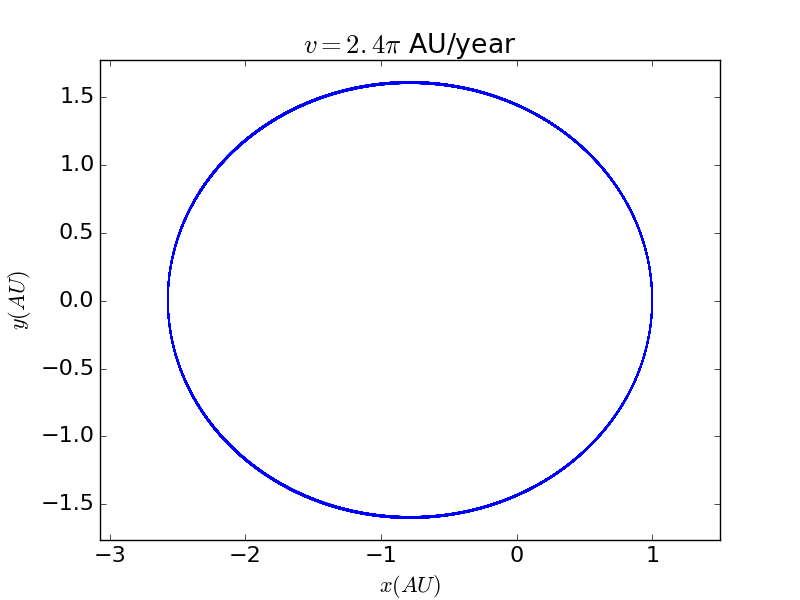
\includegraphics[width=\textwidth]{{../Programs/Output/Escape_v=1.2}.png}
	\caption{}
	\end{subfigure} 
	\begin{subfigure}[b]{0.49\textwidth}
	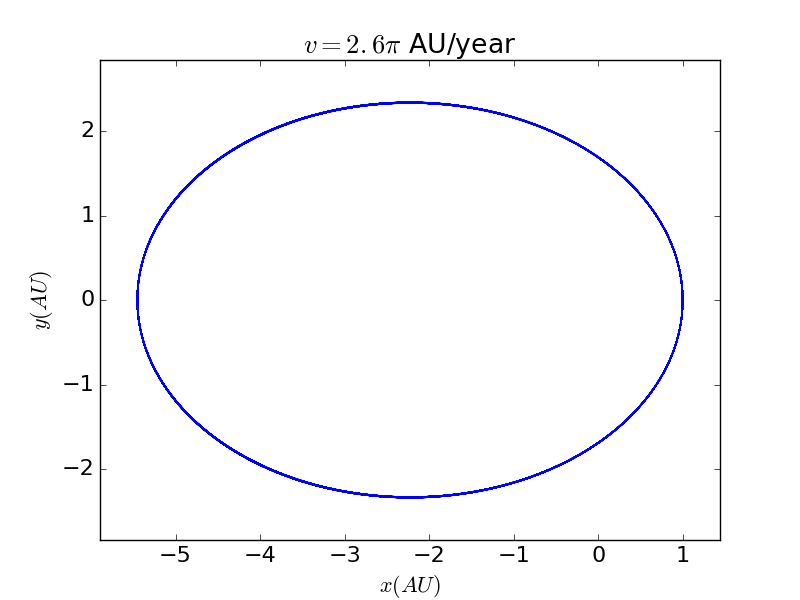
\includegraphics[width=\textwidth]{{../Programs/Output/Escape_v=1.3}.png}
	\caption{}
	\end{subfigure} 	
  	\begin{subfigure}[b]{0.49\textwidth}
	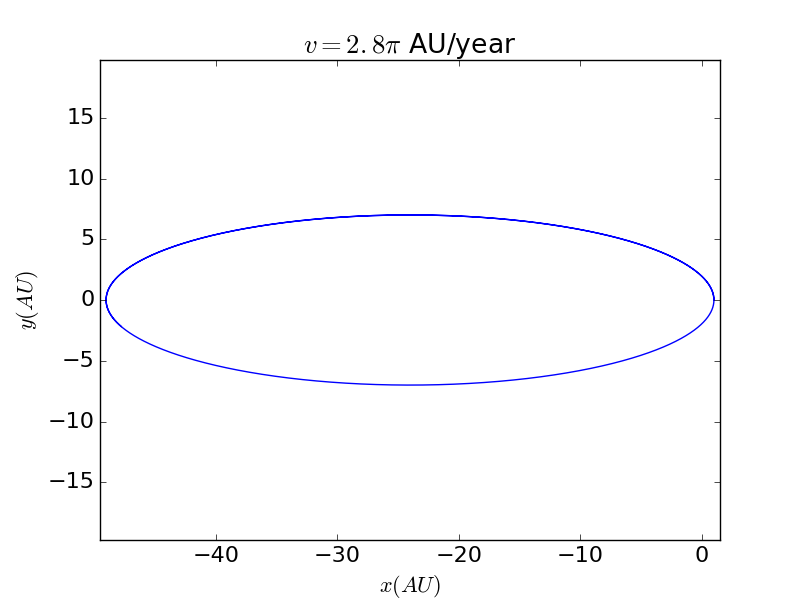
\includegraphics[width=\textwidth]{{../Programs/Output/Escape_v=1.4}.png}
	\caption{}
	\end{subfigure} 
	\begin{subfigure}[b]{0.49\textwidth}
	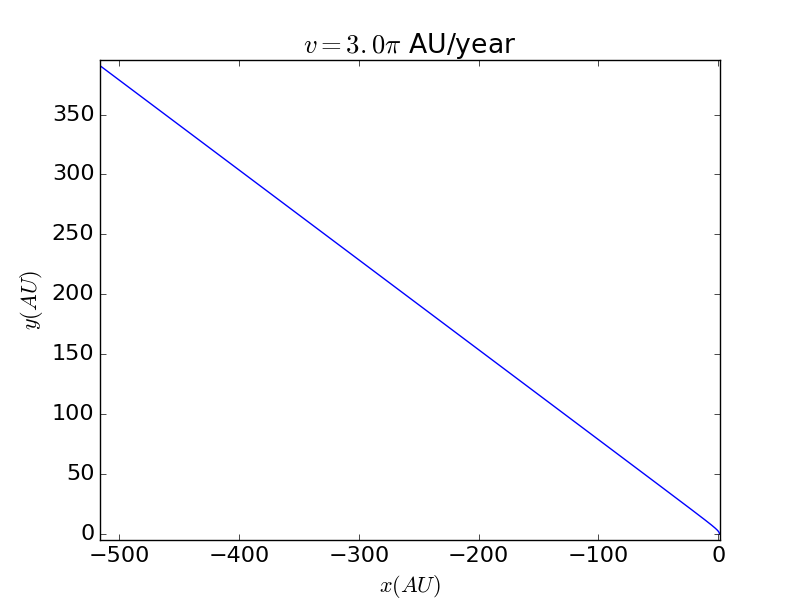
\includegraphics[width=\textwidth]{{../Programs/Output/Escape_v=1.5}.png}
	\caption{}
	\end{subfigure} 
\caption{Planet trajectories for different values of the initial velocity, simulated over 
200 years with 100,000 time steps. The initial velocity is indicated above each plot.}	
\label{fig:escape}	
\end{figure} 

The next thing we look at is a model where we let the gravitational force be given by 
\begin{align*}
F_G = \frac{GM_{\odot}M_{\text{Earth}}}{r^{\beta}}, 
\end{align*}
where $\beta \in [2,3]$. Results for $\beta$ equal to $2.5$, $2.9$, $2.99$ and $3$ are shown in 
Figure \ref{fig:modified}. We can see that for $\beta=2.5$ the system still looks nice and stable, 
but as $\beta$ creeps towards three the system starts to loose the stability, and when $\beta=3$ the Sun is 
no longer able to keep the planet in orbit, and it starts spiralling out into space. 

\begin{figure}[ht!]
\centering 
  	\begin{subfigure}[b]{0.49\textwidth}
	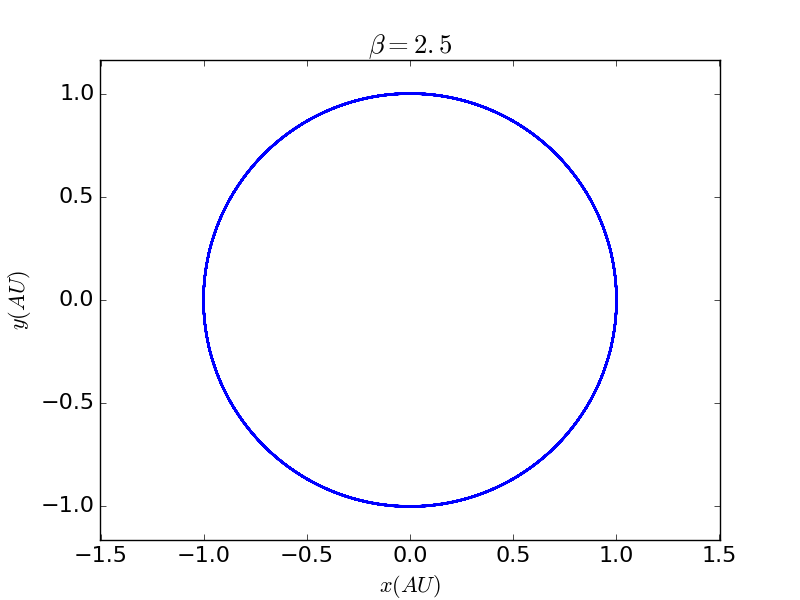
\includegraphics[width=\textwidth]{{../Programs/Output/Modified_gravity_beta=2.5}.png}
	\caption{}
	\end{subfigure} 
	\begin{subfigure}[b]{0.49\textwidth}
	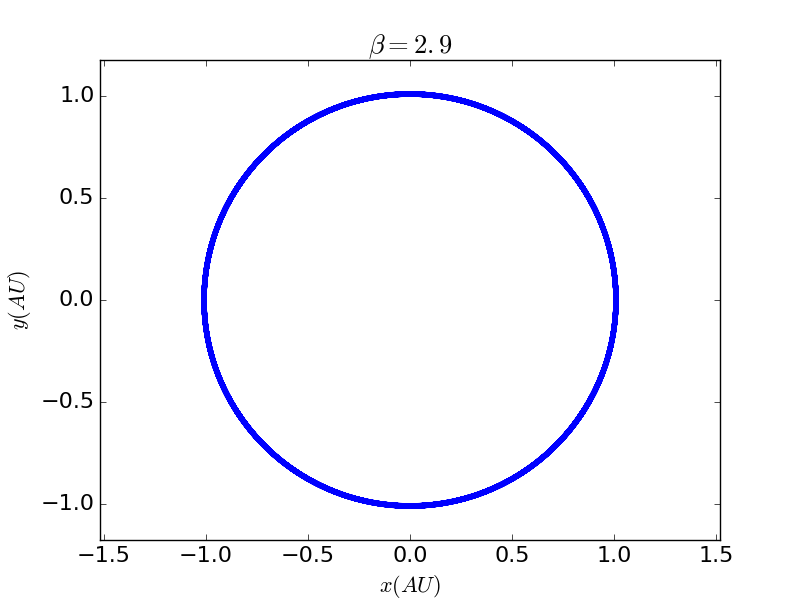
\includegraphics[width=\textwidth]{{../Programs/Output/Modified_gravity_beta=2.9}.png}
	\caption{}
	\end{subfigure} 	
  	\begin{subfigure}[b]{0.49\textwidth}
	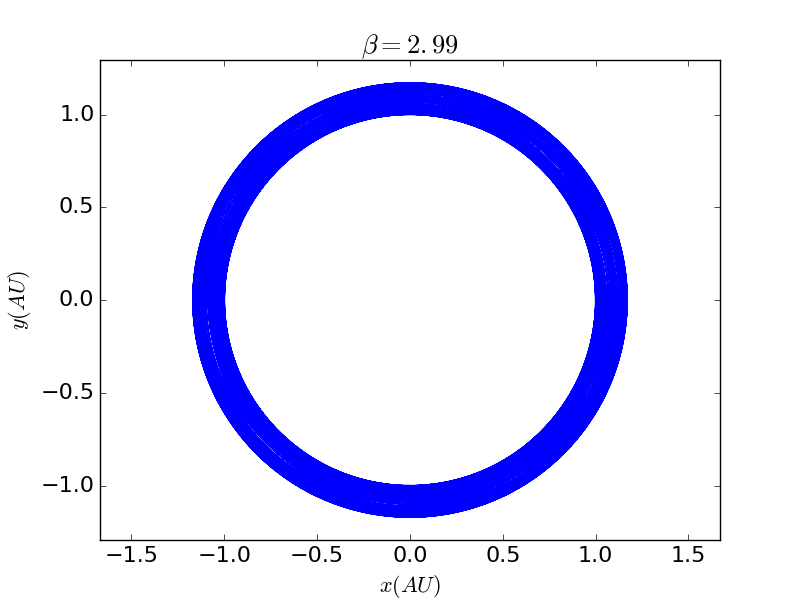
\includegraphics[width=\textwidth]{{../Programs/Output/Modified_gravity_beta=2.99}.png}
	\caption{}
	\end{subfigure} 
	\begin{subfigure}[b]{0.49\textwidth}
	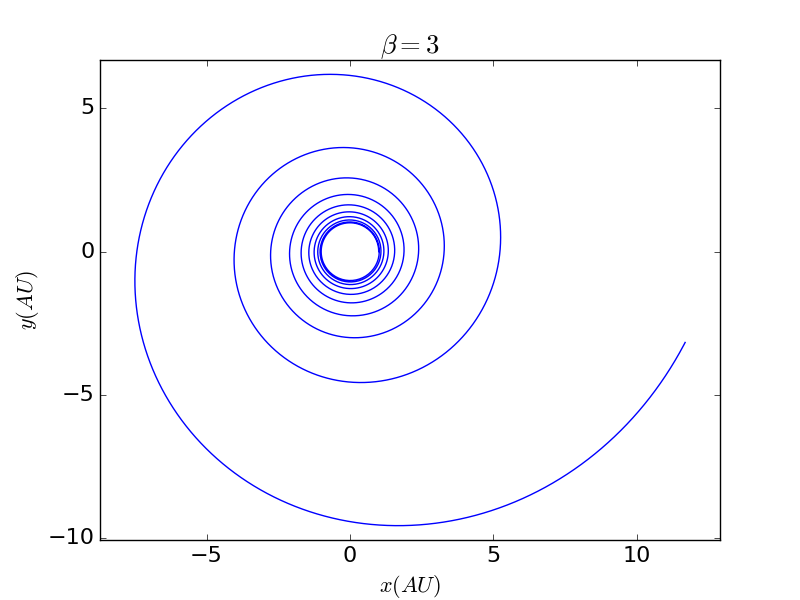
\includegraphics[width=\textwidth]{{../Programs/Output/Modified_gravity_beta=3}.png}
	\caption{}
	\end{subfigure} 
\caption{Planet trajectories with various modifications of the gravitational force, simulated over 
$100$ years with $10,000$ time steps.}	
\label{fig:modified}	
\end{figure} 

\subsection{Three-body problem}

We have now tested and played with our programs by studying one planet (i.e. the Earth) orbiting the 
Sun. Now we would like to add other planets, starting with the heaviest, namely Jupiter. Since we have 
written an object oriented code it is quite trivial to do this. We assume the motion to be co-planar, 
so we stick to studying the system in only two dimensions, and we start by considering initial velocities 
leading to circular motion, as previously. The results of this is shown in Figure \ref{fig:threebody}, 
where the simulation runs over $20$ years, using $1,000$ and $100,000$ time steps. Note that using only 
$1,000$ time steps over $20$ years mean only $50$ time steps per year, showing that the VV algorithm 
is impressively stable. The Earth orbits seems in this figure seems to be very similar to the one 
obtained with the binary system. There is however a slight difference shown in Table 
\ref{tab:earth_positions}.  

In Figure \ref{fig:massive_jupiter} we have tried to increase the mass of Jupiter with factor of $10$ and 
$1000$. We see that when making Jupiter $10$ times heavier the system is still stable, while when we 
increase by a factor of $1000$ (i.e. making Jupiter as heavy as the Sun) the system is no longer stable. 

\begin{figure}[ht!]
\centering 
  	\begin{subfigure}[b]{0.49\textwidth}
	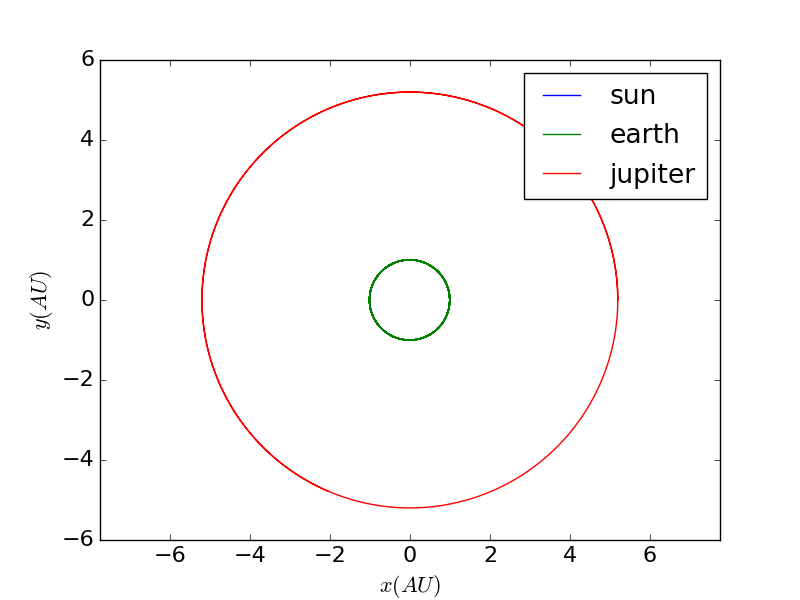
\includegraphics[width=\textwidth]{{../Programs/Output/ThreeBody_n=1000}.png}
	\caption{$1,000$ time steps.}
	\end{subfigure} 
	\begin{subfigure}[b]{0.49\textwidth}
	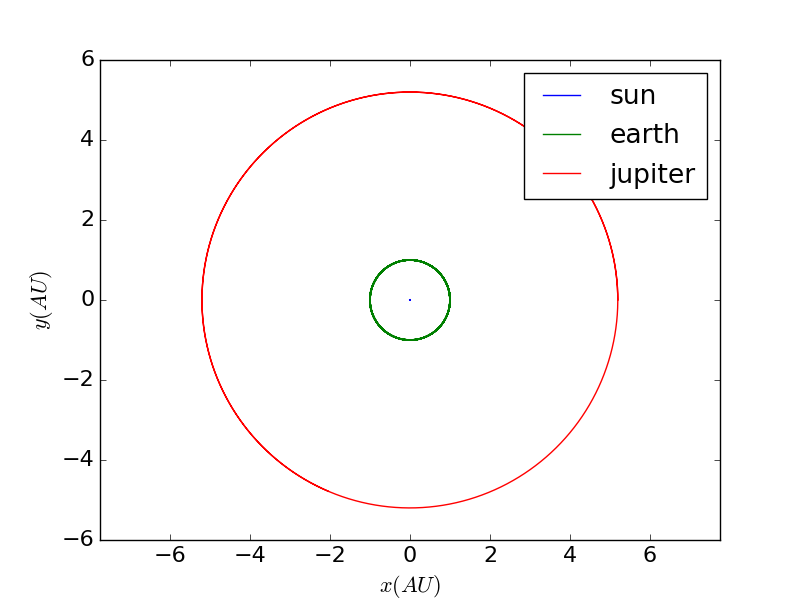
\includegraphics[width=\textwidth]{{../Programs/Output/ThreeBody_n=100000}.png}
	\caption{$100,000$ time steps.}
	\end{subfigure} 	
\caption{The three body system with the Sun, the Earth and Jupiter simulated over $20$ years with 
different number of time steps, showing that the VV algorithm is impressively stable.}	
\label{fig:threebody}
\end{figure}

\begin{figure}[ht!]
\centering 
  	\begin{subfigure}[b]{0.49\textwidth}
	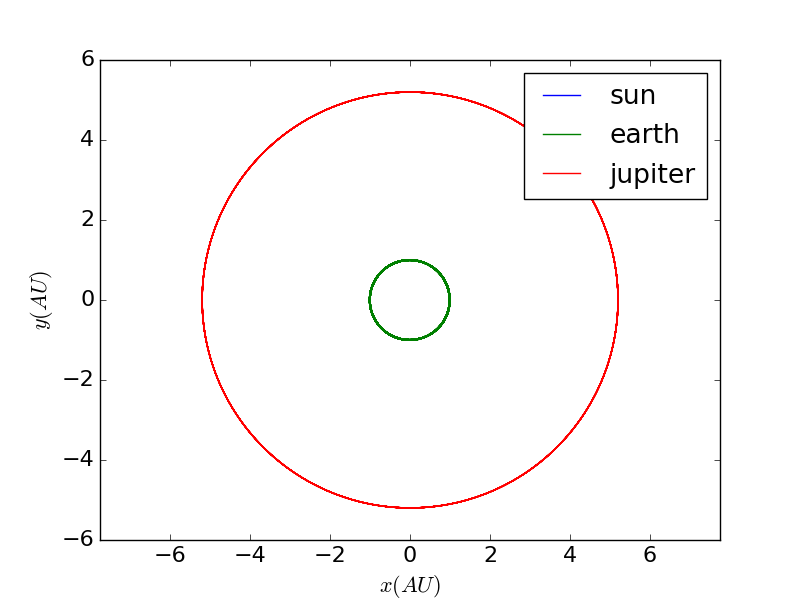
\includegraphics[width=\textwidth]{{../Programs/Output/ThreeBody_mJ=10_n=100000}.png}
	\caption{}
	\end{subfigure} 
	\begin{subfigure}[b]{0.49\textwidth}
	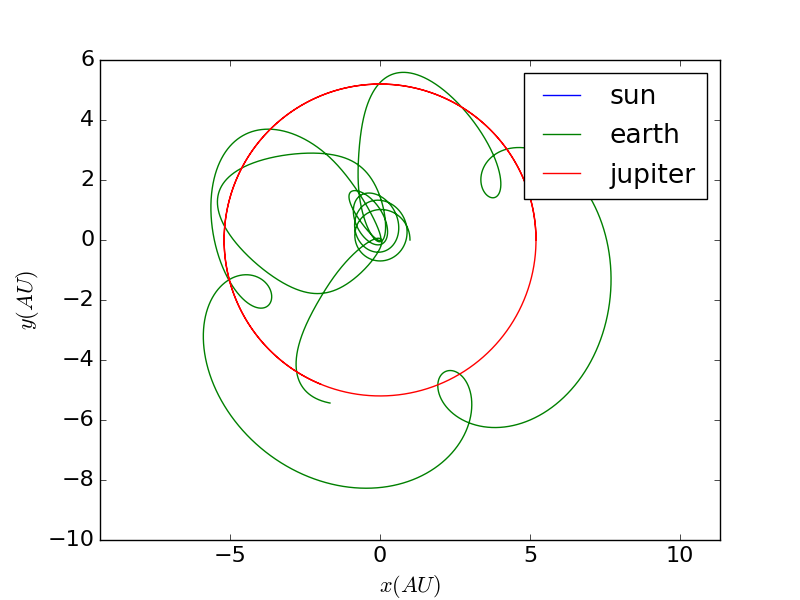
\includegraphics[width=\textwidth]{{../Programs/Output/ThreeBody_mJ=1000_n=100000}.png}
	\caption{}
	\end{subfigure} 			
\caption{Trajectories of Earth and Jupiter when the mass of Jupiter is increased by a factor of $10$ in 
(a) and a factor of $1,000$ in (b). The simulation runs over $100$ years in (a) and $20$ years in (b).}	
\label{fig:massive_jupiter}
\end{figure}

Our next step is to also set the Sun in motion, and choose the origin to be the center-of-mass, rather 
than the position of the Sun. We give the also give the Sun an initial velocity such that the total 
momentum of the system is zero, which ensures that the center-of-mass remains fixed. The resulting plots 
are shown in Figure \ref{fig:threebody_CM}, where we have zoomed in on the Sun in Figure 
\ref{fig:sun_motion}. (Notice also that the radius of the orbit of the Sun is $\sim0.005$ AU, which is 
about the same as the radius of the Sun \cite{Solar Radius}.) Comparing the orbits of the Earth and 
Jupiter with Figure \ref{fig:threebody} there is no visible difference, meaning that keeping the Sun 
fixed in the origin is a good approximation.
However, in Table \ref{tab:earth_positions} we can see that there actually is a small difference, which 
we also would expect.  


\begin{figure}[ht!]
\centering 
 	\begin{subfigure}[b]{0.49\textwidth}
	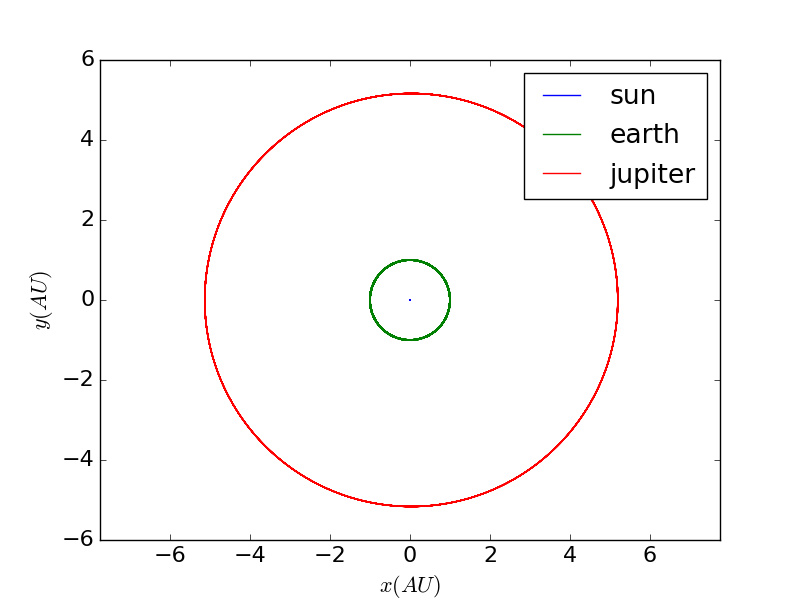
\includegraphics[width=\textwidth]{{../Programs/Output/ThreeBody_CM_100000}.png}
	\caption{}
	\end{subfigure} 
	\begin{subfigure}[b]{0.49\textwidth}
	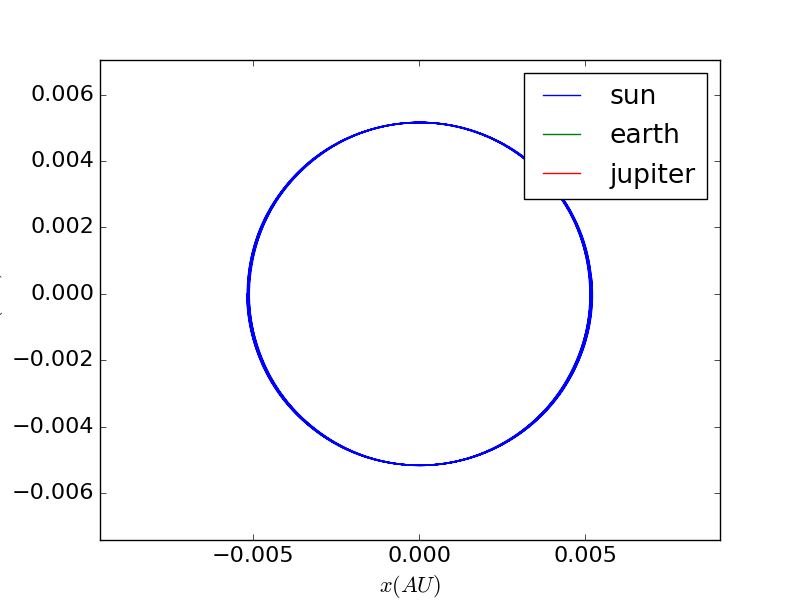
\includegraphics[width=\textwidth]{{../Programs/Output/sun_motion}.png}
	\caption{}
	\label{fig:sun_motion}	
	\end{subfigure} 
\caption{Motion of the Earth and Jupiter in (a), now also with the Sun moving. The motion of the 
Sun is shown in Figure (b). The simulation runs over $100$ years with $100,000$ time steps.}
\label{fig:threebody_CM}
\end{figure}

\begin{table}[ht!]
\caption{The maximal and minimal $x$- and $y$-positions of the Earth in different systems, found using 
simulations over $20$ years with $100,000$ time steps.}
\label{tab:earth_positions}
\begin{center}
\begin{tabular}{rcccc}   \hline\hline
System & $x_{min}$ & $y_{min}$ & $x_{max}$ & $y_{max}$ \\ \hline  
Binary (fixed Sun) & $-1.000001$ & $ -1.000000$  & $1.000000$ & $1.000000$ \\
Three-body (fixed Sun) & $-1.001280$ & $-1.000642$ & $1.000000$ & $1.000636$ \\
Three-body (moving Sun) & $-1.006822$ & $-1.006036$ & $1.005162$ & $1.005943$ \\ \hline\hline
\end{tabular}
\end{center}
\end{table}


\subsection{The solar system}

Now we move on to simulation the full solar system, with all the planets given previously in Table 
\ref{tab:planets}. The planets are initialize using NASA data taken from ref. \cite{NASA}.  
The resulting plot in three dimensions is shown in Figure \ref{fig:solarsystem}.

\begin{figure}[ht!]
\begin{center}
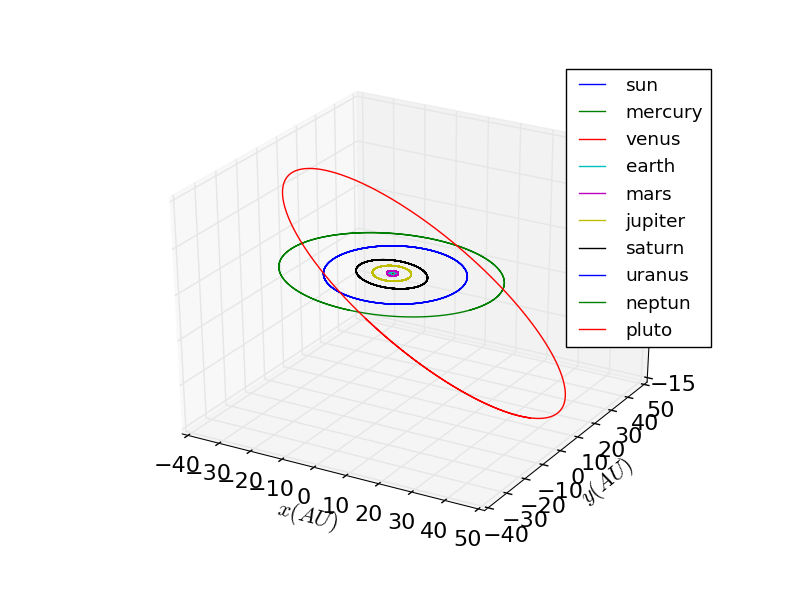
\includegraphics[width=\textwidth]{../Programs/Output/SolarSystem_3D.png}
\caption{The solar system with nine planets and the Sun simulated over $300$ years with $600,000$ time 
steps.}
\label{fig:solarsystem}
\end{center}
\end{figure}

\subsection{Perihelion precession of Mercury}

Finally, as mentioned previously, we would like to study the perihelion precession of Mercury's orbit. 
When doing this we go back to keeping the Sun fix in the origin and remove all the other planets. 
This means that by using the 
Newtonian force we should (theoretically) get no precession at all, while with the relativistic 
correction we hope to see the a precession of $\theta_p=43''\approx 0.012^{\circ}$ over one century.

The perihelion of Mercury's orbit is $0.3075$ AU, and the velocity at perihelion is $12.44$ AU/year. 
We initialize the system by putting the perihelion along the $x$-axis, so that the perihelion 
coordinates initially are given by $x_p=0.3075$ AU and $y_p=0$ AU. The angle between the perihelion 
and the $x$-axis is then given by 
\begin{align*}
\tan\theta_p = \frac{y_p}{x_p},  
\end{align*}
and this quantity is calculated and updated in the code as the years passes by, and printed out in the 
end. If the correction from General Relativity is correct we should get a final value 
$\tan\theta_p \approx 2.085\cdot 10^{-4}$. 

Since the expected perihelion angle is very small we need extremely good time resolution in order to 
see any difference between the two cases, so the simulation is done using $1$ billion time steps. 
The results are shown in Table \ref{tab:perihelion}, and they agree quite well with the observed 
perihelion precession! The slight difference can probably be blamed on round-off errors in the conversion 
between arc seconds and degrees, and possibly also on limited numerical precision in the computer.  

\begin{table}[ht!]
\caption{Comparison of Newtonian and relativistic calculation of the perihelion angle $\tan\theta_p$.}
\label{tab:perihelion}
\begin{center}
\begin{tabular}{cc} \\ \hline\hline 
& $\tan\theta_p$ \\ \hline
Newtonian & $1.062\cdot 10^{-6}$ \\
Relativistic & $2.080\cdot 10^{-4}$ \\ \hline\hline
\end{tabular}
\end{center}
\end{table}


\section{Summary and conclusions}

In this project we have simulated planetary motion by using two different methods; the forward Euler 
algorithm and the velocity Verlet algorithm. When testing and comparing these methods we found that 
velocity Verlet was a better algorithm, e.g. due to better stability and conservation of kinematic 
quantities like energy and angular momentum. 

Since we have studied several different systems we have also seen the usefulness of making an object 
oriented program. This introduced a great deal of flexibility to our programs, and made it easy to switch 
between studying the different systems, like a binary system, a three-body system and a full solar system. 
We have also experimented with for example the form of the gravitational force and the mass of Jupiter, 
and seen that the solar system becomes unstable if these are sufficiently altered. 

Finally, we also saw that, by adding a relativistic correction to the Newtonian force, we are able to 
explain the observed perihelion precession of Mercury, even though this quantity is very small.  


\begin{thebibliography}{40}

\bibitem{OOP} Dahl, Ole-Johan (2004). \textit{The Birth of Object Orientation:  the Simula
Languages} \\
\href{http://www.mn.uio.no/ifi/english/about/ole-johan-dahl/bibliography/the-birth-of-object-orientation-the-simula-languages.pdf}{http://www.mn.uio.no/ifi/english/about/ole-johan-dahl/bibliography/the-\\birth-of-object-orientation-the-simula-languages.pdf}

\bibitem{Solar Radius} Solar Radius, Wikipedia. \\ 
\href{https://en.wikipedia.org/wiki/Solar\_radius}{https://en.wikipedia.org/wiki/Solar\_radius} 
(26/10-2017)

\bibitem{NASA} Solar System Dynamics (HORIZONS Web-Interface), NASA. \\
\href{https://ssd.jpl.nasa.gov/horizons.cgi}{https://ssd.jpl.nasa.gov/horizons.cgi} (16/10-2017)


\end{thebibliography}

\end{document}

